\chapter{The Energy Efficiency of Concurrent Haskell}
In this chapter, we present an empirical study evaluating the performance and energy consumption characteristics of three thread management constructs and three data-sharing primitives of Concurrent Haskell. We start by providing a brief overview (\secref{sec:overview}) of the study and state the research questions. \secref{sec:setup} describes the benchmark we developed, the environment and the methodology we used. Sections \ref{sec:results} and \ref{sec:discussion} provides our results. Finally, \secref{sec:threats} list the threats to validity.

\section{Overview}\label{sec:overview}
Recently, the software engineering community have been showing a keen interest in researching about the development of energy-efficient software. As multicore architectures are the norm nowadays, this interest also extends for energy-efficiency from the perspective of concurrent software running on multicore architectures~\citep{trefethen:2013,ribic:2014, pinto:2014}. However, there is no much traction from the functional programming side yet. This is unfortunate as functional programming languages are seen as a good alternative for making concurrent programming less error-prone. Particularly, Haskell provides a solid foundation for building concurrent software, and we know very little about its energy behavior.

We believe that the first step to optimizing energy consumption of concurrent programs is to gain a comprehensive understanding of their energy behaviors. This chapter presents an empirical study to understand the energy behaviors of Haskell concurrent programs on multicore architectures. In particular, our study focuses on how programmer's decisions may impact energy consumption and performance. The following questions motivate our research:

\begin{enumerate}[label=\RQ{\arabic*}.]
  \item Do alternative \textit{thread management constructs} have different impacts on energy consumption?
  \item Do alternative \textit{data-sharing primitives} have different impacts on energy consumption?
  \item What is the relationship between the \textit{number of capabilities} and energy consumption?
\end{enumerate}

To answer \RQ{1}, we select three thread management constructs: \forkIO, \forkOn and \forkOS. As we saw in \secref{sec:haskell-conc}, these are the three functions we have in Haskell to spawn a new thread of execution. To answer \RQ{2}, we select three data-sharing primitives: \MVar, \TMVar and \TVar. Given these constructs, our investigation aims to understand how the energy consumption can be impacted by simply changing the concurrency primitive used in a Haskell program. Finally, to answer \RQ{3}, we explore various capabilities settings to see how it can impact energy consumption and performance on a multicore environment.


\section{Study Setup}\label{sec:setup}
In this section we describe the benchmarks that we analyzed, the infrastructure and the methodology that we used to perform the experiments.

\subsection{Benchmarks}
We selected a variety of concurrent Haskell programs to use as benchmarks in our study, listed as follows. Benchmarks \ref{bench:chameneos}-\ref{bench:spectral} are from \ac{clbg}\footnote{http://benchmarksgame.alioth.debian.org/}. \acs{clbg} is a benchmark suite aiming to compare the performance of the runtime of various programming languages. Benchmark \ref{bench:dining} is from  Rosetta Code \footnote{http://rosettacode.org/}, a code repository of solutions to common programming tasks. Benchmarks \ref{bench:tsearch}-\ref{bench:warp} were developed by us.

\begin{enumerate}
  \item \label{bench:chameneos}\chameneos: In this benchmark chameneos creatures go to a meeting place and exchange colors with a meeting partner. It encodes symmetrical cooperation between threads.

  \item \fasta:  This benchmark generates random DNA sequences and writes it in FASTA format\footnote{https://en.wikipedia.org/wiki/FASTA\_format}. The size of the generated DNA sequences is in the order of hundreds of megabytes. In this benchmark,  each worker synchronizes with the previous one to output the sub-sequences of DNA in the correct order.

  \item \knucleotide: This benchmark takes a DNA sequence and counts the occurrences and the frequency of nucleotide patterns. This benchmark employs string manipulation and hashtable updates intensively. There is no synchronization in the program besides the main thread waiting for the result of each worker.

  \item \mandelbrot: A mandelbrot is a mathematical set of points whose boundary is a distinctive and easily recognizable two-dimensional fractal shape. Mandelbrot set images are created by sampling complex numbers and determining for each one whether the result tends toward infinity when a particular mathematical operation is iterated on it. The only synchronization point in this benchmark is the main thread waiting for the result of each worker.

  \item \regex: This benchmark implements a string-based algorithm that performs multiple regular expression operations, match and replace, over a DNA sequence. The only synchronization point is the main thread waiting for the result of each worker.

  \item \label{bench:spectral}\spectral: The spectral norm is the maximum singular value of a matrix. It synchronizes the workers using a cyclic barrier.

  \item \label{bench:dining}\dining: An implementation of the classical concurrent programming problem posed by~\cite{dijkstra:1971}. The philosophers perform no work besides manipulating the forks and printing a message when eating.

  \item \label{bench:tsearch}\tsearch: A parallel text search engine. This benchmark searches for occurrences of a sentence in all text files in a directory and its sub-directories. It is based on a previous empirical study comparing STM and locks~\citep{pankratius:2011}.

  \item \label{bench:warp}\warp: Runs a set of queries against a Warp server retrieving the resulting webpages. Warp is the default web server used by the \ac{wai}, part of the Yesod Web Framework. This benchmark was inspired by the Tomcat benchmark from DaCapo~\citep{blackburn:2006}.
\end{enumerate}

We selected the benchmarks based on their diversity. For instance, \chameneos and \dining are synchronization-intensive programs. \mandelbrot and \spectral are CPU-intensive and scale well on a multicore machine. \knucleotide and \regex are CPU- and memory-intensive, while \warp is IO-intensive. \tsearch combines IO and CPU operations, though much of the work it performs is CPU-intensive. \fasta is peculiar in that is CPU-, memory-, synchronization- and IO-intensive.

Also, some benchmarks have a fixed number of workers (\chameneos, \knucleotide, \regex, and \dining) and others spawn as many workers as the number of capabilities (\fasta, \mandelbrot, \spectral, \tsearch and \warp). For the \dining benchmark, it is possible to establish prior to execution the number of workers.

\subsection{Experimental Environment}
For our study, all experiments were conducted on a machine with 2x10-core Intel Xeon E5-2660 v2 processors (Ivy Bridge microarchitecture), 2.20 GHz, with 256GB of DDR3 1600MHz memory. It has three cache levels (L1, L2, L3): L1 with 32KB per core, L2 with 256KB per core, and L3 with 25MB per socket (Smart cache). This machine runs the Ubuntu Server 14.04.3 LTS (kernel 3.19.0-25) operating system, \acs{ghc} 7.10.2, and our modified Criterion based on version 1.1.0 of the official release.

All experiments were performed with no other load on the OS. We conform to the default settings of the operating system. For each benchmark, we used the same compilation and runtime flags employed in the original benchmark suites. This is important to preserve the same performance characteristics as intended by the implementers. Both the energy consumption and the performance is measured by Criterion.

\subsection{Methodology}
Most of the benchmarks we used were implemented in its respective suite using a single thread management construct and a single data-sharing primitive. For the ones from \acs{clbg}, for example, they were implemented using \forkIO and \MVar. In order to analyze the impact of both thread management constructs and data-sharing primitives, we manually refactored each benchmark to create new \emph{variants} using different constructs. Changing the thread management construct is a straightforward process. The functions have almost the same signature. The only exception is \forkOn that requires an extra argument representing in which capability the thread will run. For this study, we distributed the threads evenly among the capabilities when using \forkOn. However, changing the data-sharing primitive is not always simple as a \TVar have a quite different semantics when compared to an \MVar. To properly do this refactoring, we used the techniques proposed by~\cite{soares-neto:2014} to refactor the benchmarks to use STM.

As a result of this process, each benchmark has up to 9 distinct variants covering a number of different combinations of both thread management constructs and data-sharing primitives. However, it is important to note that there are some cases like \dining where not all possible combinations were created. In this particular implementation, the shared variable is also used as a condition-based synchronization mechanism. In such cases, we did not create \TVar variants as \TMVar mimics exactly this behavior, while using Haskell's STM. In other benchmarks like \tsearch and \warp, we changed only the thread management construct as they are complex applications and it would not be straightforward to change the synchronization primitives without introducing potential bugs.

In the end, each variant we created is represented by a standalone executable. This executable is a Criterion microbenchmark that performs the experiment by calling the original program entry point multiple times. We run this executable nine times, each one changing the number \texttt{N} of capabilities used by the runtime system. We used the following values for \texttt{N}: $\{1, 2, 4, 8, 16, 20, 32, 40, 64\}$. Where 20 and 40 are the number of physical and virtual cores, respectively.

In \appref{ap:benchmark}, we provide an example of one of the benchmarks we used. We show the description of the problem that this benchmark solves and the implementation of each variant we generated to use in this study. It can also be accessed on GitHub at \url{http://github.com/green-haskell/concurrency-benchmark}. In this repository, we made publicly available the implementation of all benchmarks variants as well as the scripts and instructions necessary to replicate this experiment.


\section{Study Results}\label{sec:results}
In this section, we report the results of our experiments with concurrent Haskell programs. The results are presented in Figures \ref{fig:conc_bench1}, \ref{fig:conc_bench2} and \ref{fig:conc_bench3}. Here, the odd rows are energy consumption results, while the even rows are the corresponding running time results. We omitted the experiments using 64 capabilities in order to make the charts more readable. The charts including this configuration as well as all the data and source code used in this study are available at \href{http://green-haskell.github.io/}{green-haskell.github.io}.
\newline

\begin{figure*}[tp]
\caption{Energy and Time charts for \chameneos, \dining, \fasta and \knucleotide}
\centering
$
\begin{array}{ccc}
 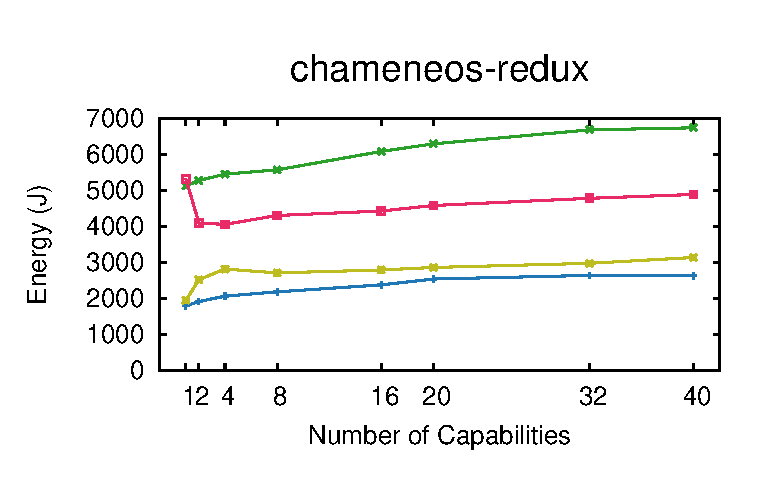
\includegraphics[width=.48\textwidth]{images/conc_bench/chameneos-redux-energy} &
 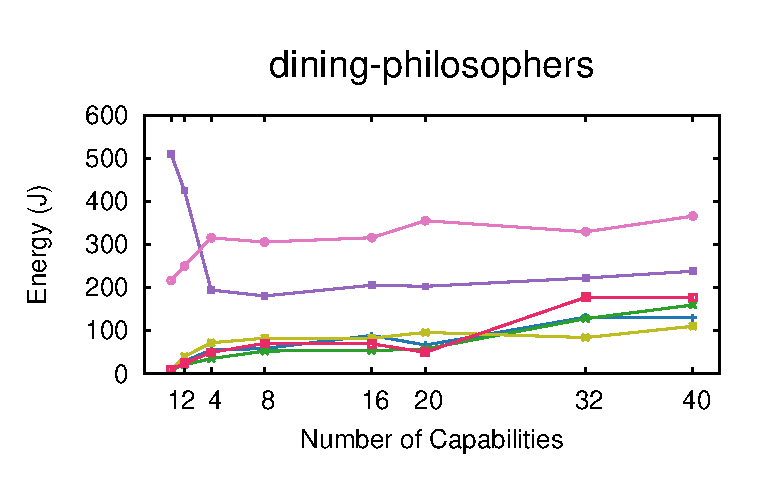
\includegraphics[width=.48\textwidth]{images/conc_bench/dining-philosophers-energy} \\
 \\

 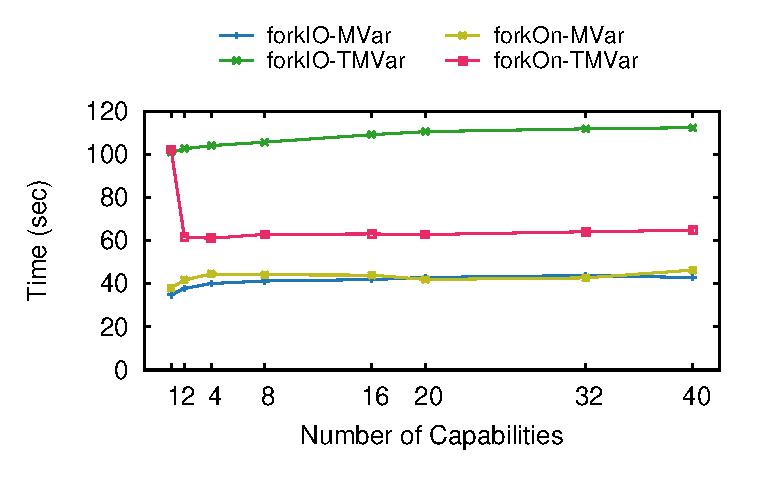
\includegraphics[width=.48\textwidth]{images/conc_bench/chameneos-redux-time} &
 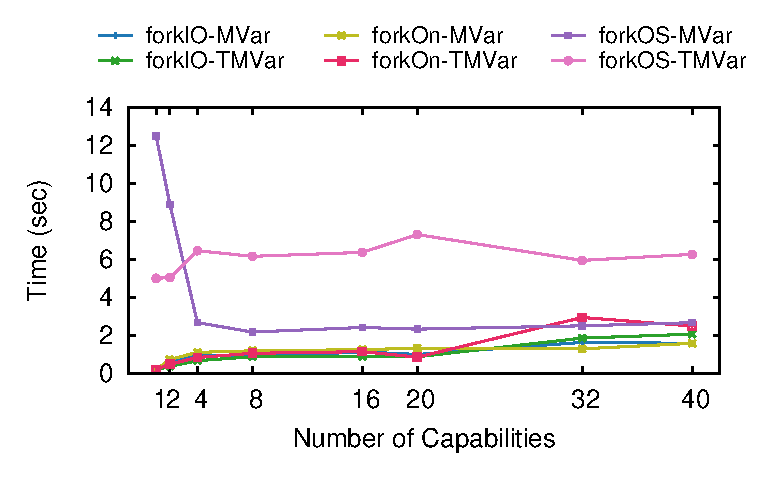
\includegraphics[width=.48\textwidth]{images/conc_bench/dining-philosophers-time} \\

 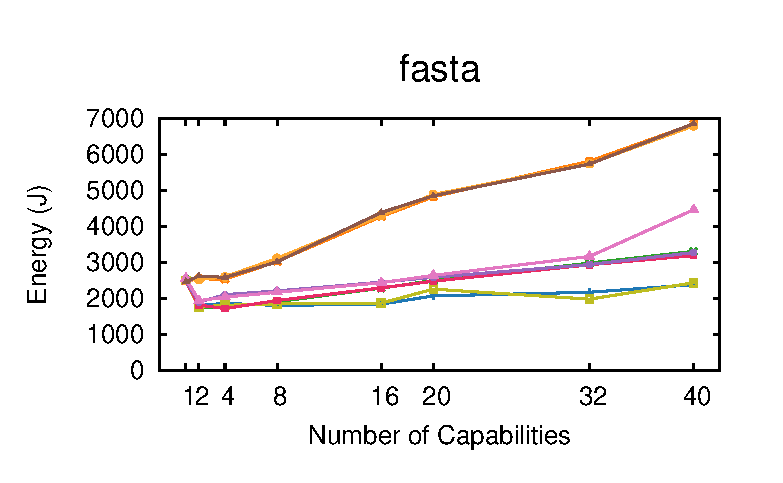
\includegraphics[width=.48\textwidth]{images/conc_bench/fasta-energy} &
 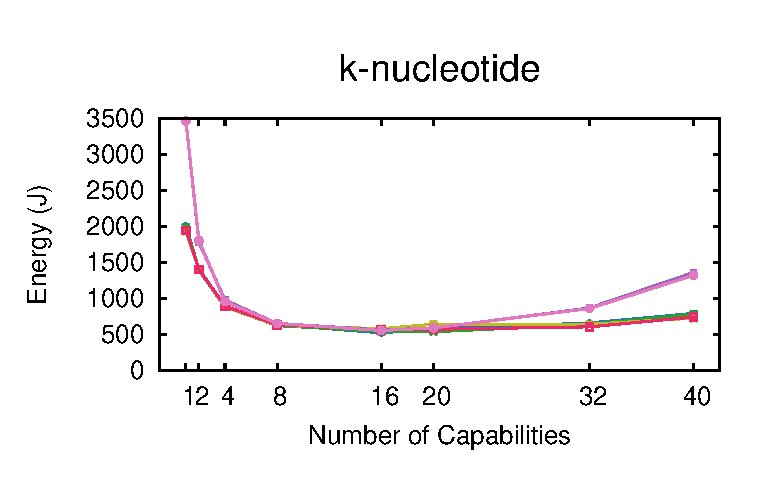
\includegraphics[width=.48\textwidth]{images/conc_bench/k-nucleotide-energy}  \\

 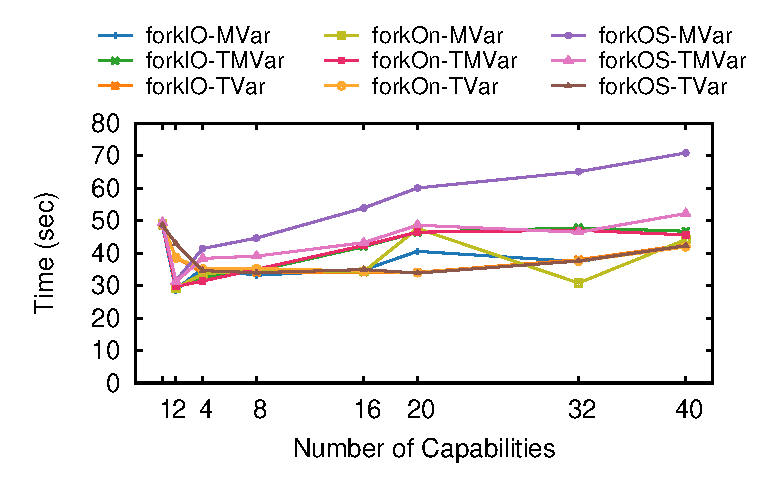
\includegraphics[width=.48\textwidth]{images/conc_bench/fasta-time} &
 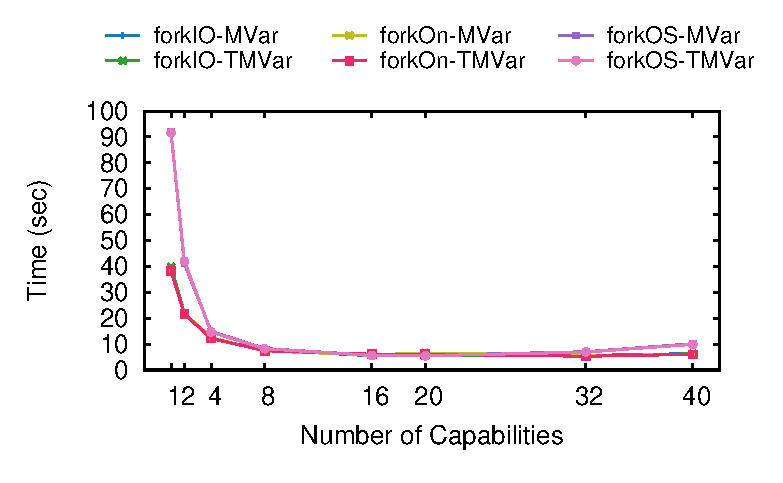
\includegraphics[width=.48\textwidth]{images/conc_bench/k-nucleotide-time}  \\
\end{array}
$
\footnotesize{Source: Made by the author.}
\label{fig:conc_bench1}
\end{figure*}

\begin{figure*}[tp]
\caption{Energy and Time charts for \mandelbrot, \regex, \spectral and \tsearch}
\centering
$
\begin{array}{ccc}
 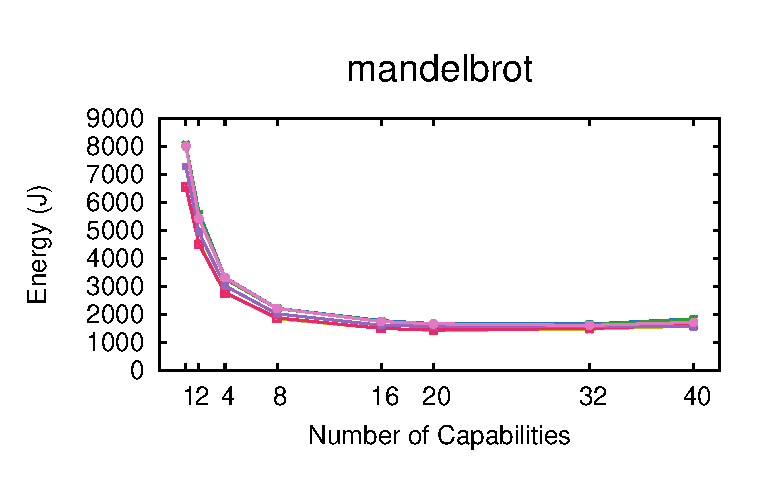
\includegraphics[width=.48\textwidth]{images/conc_bench/mandelbrot-energy} &
 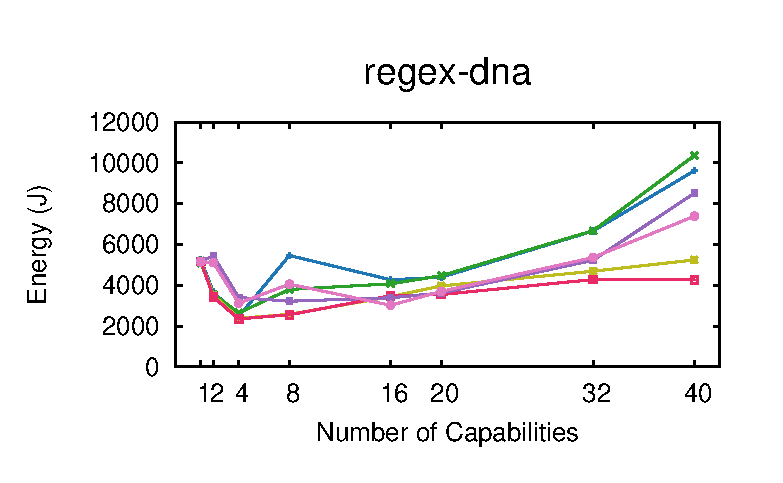
\includegraphics[width=.48\textwidth]{images/conc_bench/regex-dna-energy} \\

 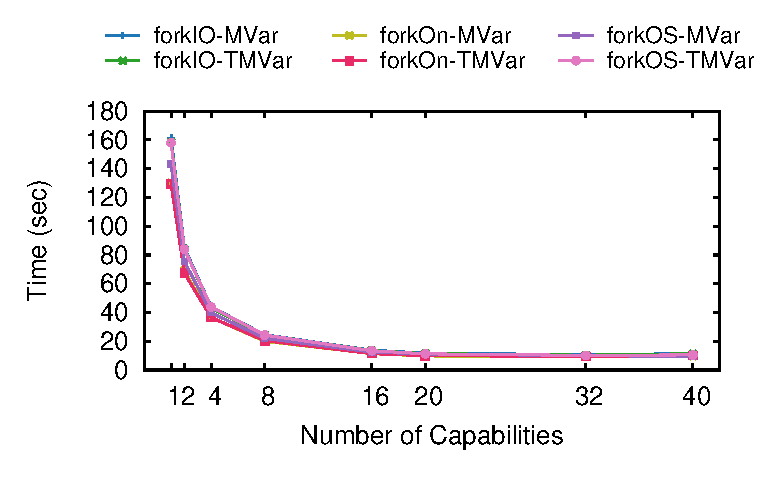
\includegraphics[width=.48\textwidth]{images/conc_bench/mandelbrot-time} &
 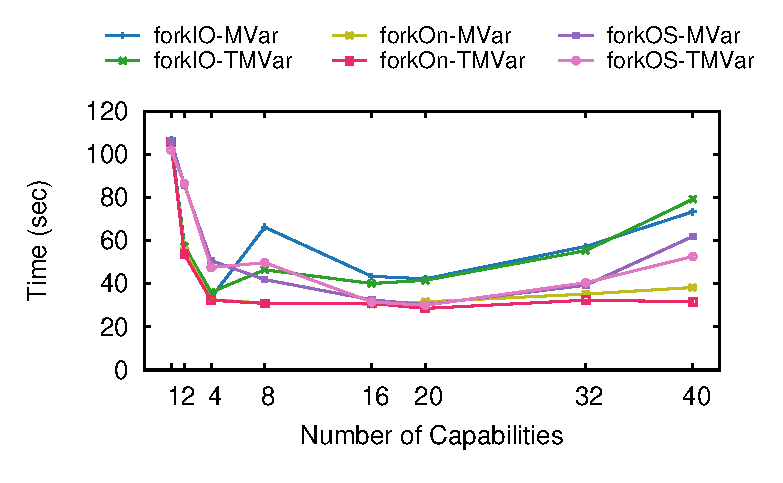
\includegraphics[width=.48\textwidth]{images/conc_bench/regex-dna-time} \\
 \\

 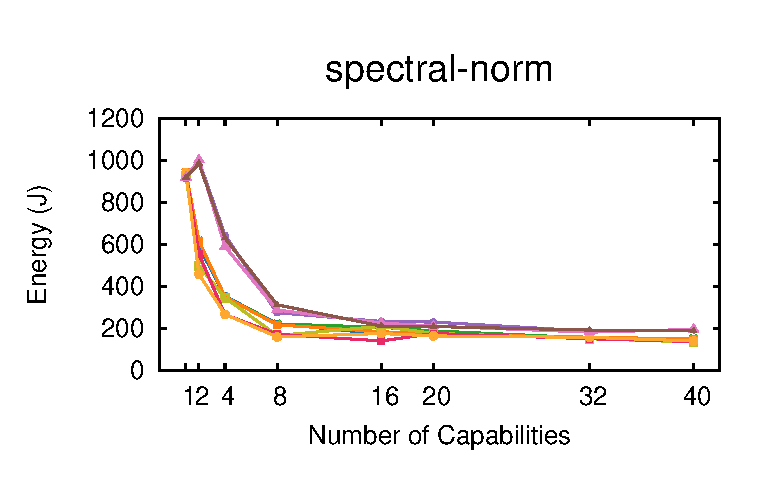
\includegraphics[width=.48\textwidth]{images/conc_bench/spectral-norm-energy} &
 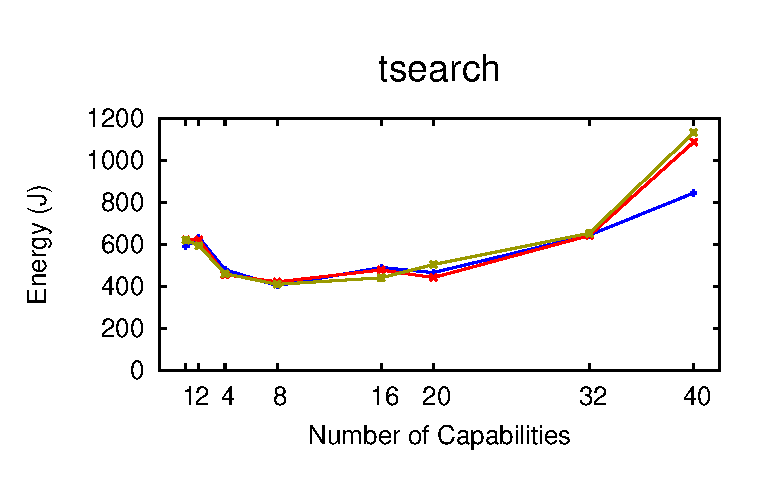
\includegraphics[width=.48\textwidth]{images/conc_bench/tsearch-energy} \\

 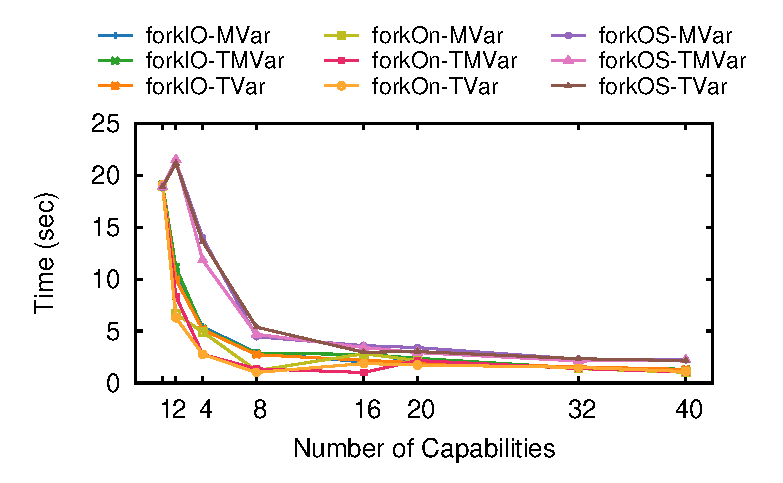
\includegraphics[width=.48\textwidth]{images/conc_bench/spectral-norm-time} &
 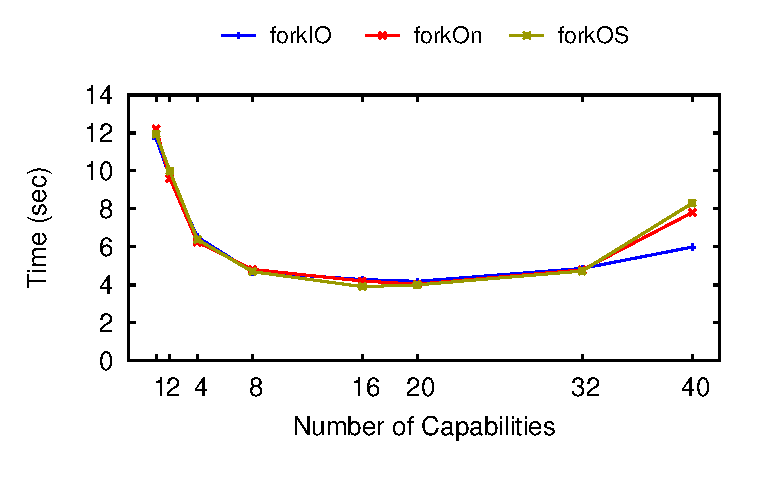
\includegraphics[width=.48\textwidth]{images/conc_bench/tsearch-time} \\
\end{array}
$
\footnotesize{Source: Made by the author.}
\label{fig:conc_bench2}
\end{figure*}

\begin{figure*}[tp]
\caption{Energy and Time charts for \warp}
\centering
$
\begin{array}{c}
 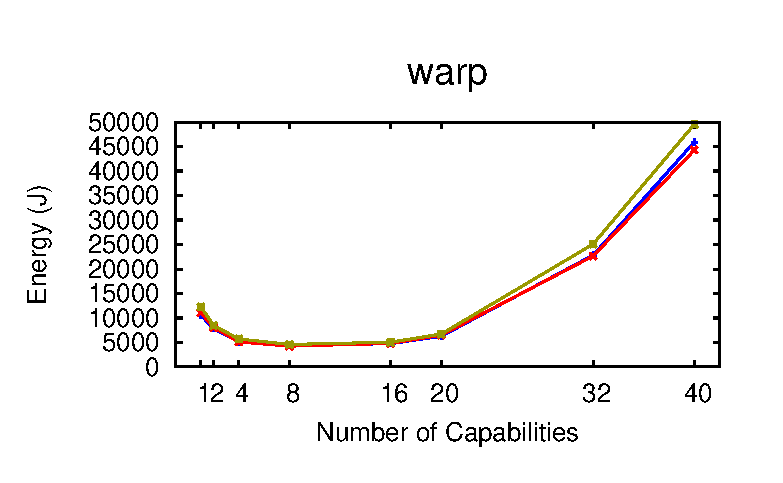
\includegraphics[width=.48\textwidth]{images/conc_bench/warp-energy} \\
 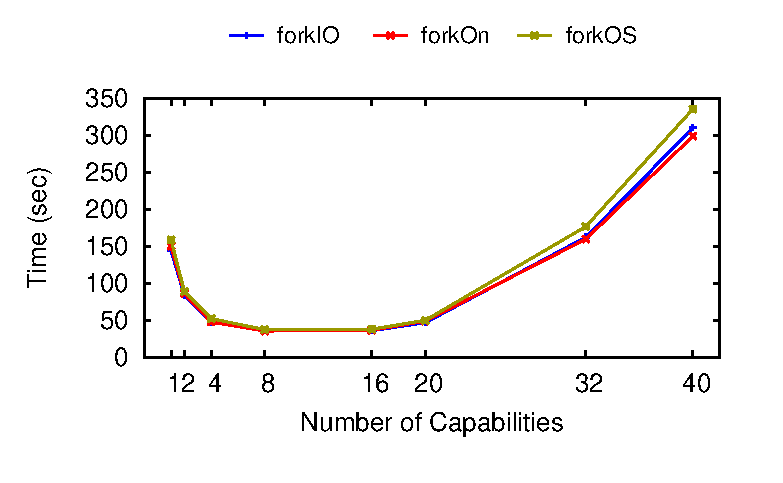
\includegraphics[width=.48\textwidth]{images/conc_bench/warp-time} \\
\end{array}
$
\\
\footnotesize{Source: Made by the author.}
\label{fig:conc_bench3}
\end{figure*}

\state{Small changes can produce big savings.} One of the main findings of this study is that simple refactorings such as switching between thread management constructs can have considerable impact on energy usage. For example, in \spectral, using \forkOn instead of \forkOS with \TVar can save between 25 and 57\% energy, for a number of capabilities ranging between 2 and 40. Although the savings vary depending on the number of capabilities, for \spectral \forkOn exhibits lower energy usage independently of this number. For \mandelbrot, variants using \forkOS and \forkOn with \MVar exhibited consistently lower energy consumption than ones using \forkIO, independently of the number of capabilities. For the \forkOS variants, the savings ranged from 5.7 to 15.4\% whereas for \forkOn variants the savings ranged from 11.2 to 19.6\%.

This finding also applies to data sharing primitives. In \chameneos, switching from \TMVar to \MVar with \forkOn can yield energy savings of up to 61.2\%. Moreover, it is advantageous to use \MVar independently of the number of capabilities. In a similar vein, in \fasta, going from \TVar to \MVar with \forkIO can produce savings of up to 65.2\%. We further discuss the implications of this finding in \secref{sec:discussion}.
\newline

\state{Faster is not always greener.} Overall, the shapes of the curves in Figures \ref{fig:conc_bench1}, \ref{fig:conc_bench2} and \ref{fig:conc_bench3} are similar. Although, for 6 of our 9 benchmarks, in at least two variants of each one, there are moments where faster running time leads to a higher energy consumption. For instance, in the \forkOn-\TMVar variant of \regex, the benchmark is 12\% faster when varying the number of capabilities from 4 to 20 capabilities. But at the same time, its energy consumption increases by 51\% . Also, changing the number of capabilities from 8 to 16 in the \forkIO variant of \tsearch makes it 8\% faster and 22\% less energy-efficient.

In one particular benchmark, \fasta, we had strongly divergent results in terms of performance and energy consumption for some of the variants. For this benchmark, the variants  employing \TVar outperformed the ones using \TMVar and \MVar. For example, when using a number of capabilities equal to the number of physical cores of the underlying machine (20), the \forkOS-\TVar variant was 43.7\% faster than the \forkOS-\MVar one. At the same time, the \TVar variants exhibited the worst energy consumption. In the aforementioned configuration, the \forkOS-\TVar variant consumed 87.4\% more energy.
\newline

\state{There is no overall winner.} Overall, no thread management construct or data sharing primitive, or combination of both is the best. For example, the \forkIO-\TMVar variant is one of most energy-efficient for \dining. The \forkOS-\TMVar variant consumes more than 6 times more energy. However, for the \chameneos benchmark, the \forkIO-\TMVar variant consumes 2.4 times more energy than the best variant, \forkIO-\MVar. This example is particularly interesting because these two benchmarks have similar characteristics. Both \dining and \chameneos are synchronization-intensive benchmarks and both have a fixed number of worker threads. Even in a scenario like this, using the same constructs can lead to discrepant results.
\newline

\state{Choosing more capabilities than available CPUs is harmful.} The performance of most benchmarks is severely impaired by using more capabilities than the number of available CPUs. In \chameneos, for example, moving from 40 to 64 capabilities can cause a 13x slowdown. This suggests that the Haskell runtime system was not designed to handle cases where capabilities outnumber CPU cores. In fact, this assumption makes sense as the official GHC documentation recommends the number of capabilities to match the number of CPU cores. However, the documentation leaves as an open question if virtual cores should be counted. In our experiments, the performance almost never improves after 20 capabilities. So developers should be careful when using more capabilities than available physical CPU cores as it can degrade performance.


\section{Discussion}\label{sec:discussion}
Generally, especially in the sequential benchmarks, high performance is a proxy for low energy consumption. A study we published \citep{lima:2016} highlighted this for a number of different data structure implementations and operations. Concurrency makes the relationship between performance and energy less obvious, however. Also, there are clear benefits in employing  different thread management constructs and data-sharing primitives. This section examines this in more detail.

Switching between thread management construct is very simple in Haskell. Functions \forkOn, \forkIO, and \forkOS take a computation of type \IO as parameter and produce results of the same type. Thus, the only difficulty is in determining on which capability a thread created via \forkOn will run. This is good news for developers and maintainers. Considering the 7 benchmarks where we implemented variants using different data sharing primitives, in 5 of them the thread management construct had a stronger impact on energy usage than the data sharing primitives. Furthermore, in these 5 benchmarks and also in \warp it is clearly beneficial to switch between thread management constructs.

Alternating between data sharing primitives is not as easy, but still not hard, depending on the characteristics of the program to be refactored. Going from \MVar to \TMVar and back is straightforward because they have very similar semantics. The only complication is that, since functions operating on \TMVar produce results of type \STM, calls to these functions must be enclosed in calls to \atomically to produce a result of type \IO. Going from \MVar to \TVar and back is harder, though. If a program using \MVar does not require condition-based synchronization, it is possible to automate this transformation in a non-application-dependent manner~\citep{soares-neto:2014}. If condition-based synchronization is necessary, such as is the case with the \dining benchmark, the semantic differences between \TVar and \MVar make it necessary for the maintainer to understand details of how the application was constructed.

In spite of the absence of an overall winning thread management construct or data-sharing primitive, we can identify a few cases where {\em a specific approach excels under specific conditions}. For instance, we can see that in both \mandelbrot and \spectral, \forkOn has a slightly better performance than \forkIO and \forkOS. In \mandelbrot, the \forkOn variants are around 20\% more energy-efficient than the \forkIO variants. In \spectral, \forkOn can be up to 2x greener than \forkOS. These two benchmarks are both CPU-intensive. They also create as many threads as the number of capabilities. In a scenario such as this, a computation-heavy algorithm with few synchronization points, keeping each thread executing in a dedicated CPU core is beneficial for the performance. This is precisely what \forkOn does.

Although there is no overall winner, there is a more or less clear loser, when thread management construct have a strong impact on energy: \forkOS. In only one of the benchmarks the \forkOS variants did not have the worst energy consumption and worst performance: \regex. According to the Haskell documentation\footnote{https://hackage.haskell.org/package/base-4.8.1.0/docs/Control-Concurrent.html\#v:forkOS}: \emph{"Using forkOS instead of forkIO makes no difference at all to the scheduling behavior of the Haskell runtime system".} If that is the case, the extra time and energy consumption stem from the need to switch OS threads to execute work passed to a call to \forkOS. This overhead does not exist for \forkOn and \forkIO.


\section{Threats to Validity}\label{sec:threats}
This work focused on the Haskell programming language. It is possible that its results do not apply to other functional programming languages, especially considering that Haskell is one of the few lazy programming languages in existence. Moreover, we analyzed only the data structures available in the Edison library and a subset of Haskell's constructs for concurrent and parallel programming. It is not possible to extrapolate the results to other data structure implementations or to alternative constructs for concurrent and parallel execution. Nonetheless, our evaluation comprised a large number of experimental configurations that cover widely-used constructs of the Haskell language.

It is not possible to generalize the results of this study to other hardware platforms for which Haskell programs can be compiled. Factors such as operating system scheduling policies~\citep{yuan:2003} and processor and interconnect layouts~\citep{solernou:2013} can clearly impact the results. We take a route common in experimental programming language research, by constructing experiments over representative system software and hardware, and the results are empirical by nature. To take a step further, we have re-executed the experiments in additional hardware configurations. The primary goal is to understand the stability and portability of our results. We ran some of the benchmarks on another machine, a 4-core Intel i7-3770 (IvyBridge) with 8 GB of DDR 1600 runing Ubuntu Server 14.04.3 LTS (kernel 3.19.0-25) and GHC 7.10.2. \figref{fig:other-machine-conc} shows the results of \mandelbrot running on this i7 machine. The results show analogous trends in which the curves have similar shapes to the results of \figref{fig:conc_bench2}. The same trend can be observed for the remaining benchmarks.

\begin{figure}[t]
\caption{Energy and Time charts on Alternative Platform}
\centering
$
\begin{array}{cc}
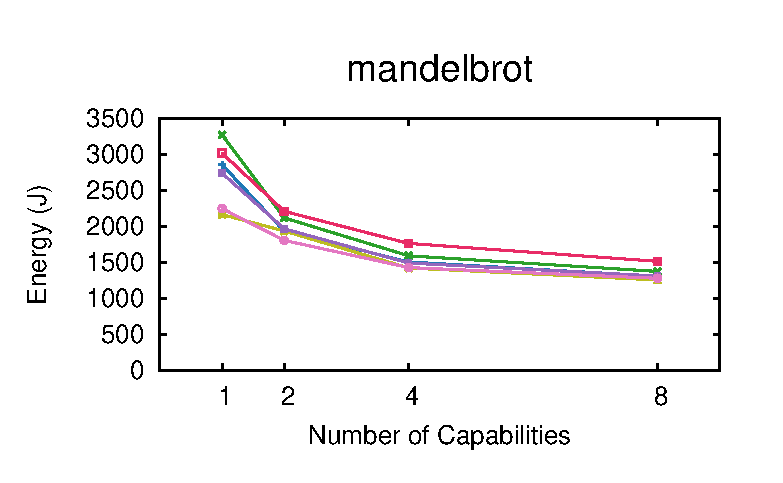
\includegraphics[width=0.47\linewidth]{images/conc_bench/mandelbrot-i7-energy} &
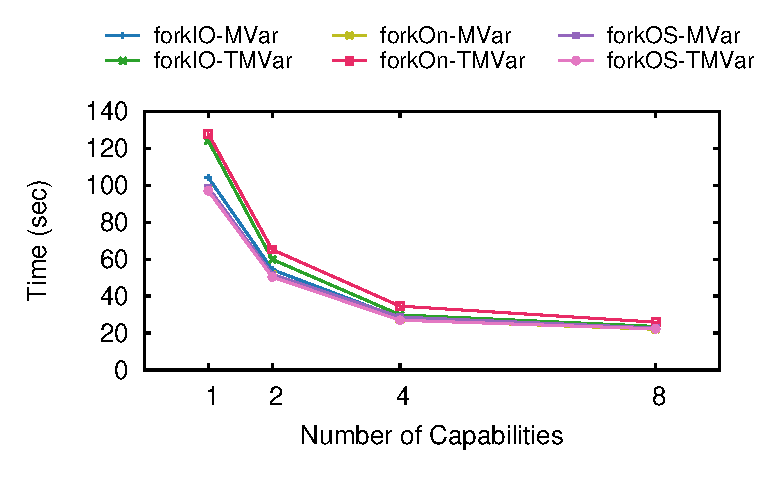
\includegraphics[width=0.47\linewidth]{images/conc_bench/mandelbrot-i7-time} \end{array}
$
\footnotesize{Source: Made by the author.}
\label{fig:other-machine-conc}
\end{figure}

It is also not possible to generalize the results to other versions of GHC. Changes in the runtime system, for example, can lead to different results. This work also did not explore the influence of the various compiler and runtime settings of GHC. As the options range from GC algorithms to scheduling behaviour, it can have a significant impact on performance, especially for concurrency. For the benchmarks we developed, we used the default settings of GHC. For the ones from CLBG, we used the same settings used there to preserve the performance characteristics intended by the developers.

One further threat is related to our measurement approach We have employed RAPL to measure energy consumption. Thus, the results could be different for external measurement equipment. Nonetheless, previous work~\citep{hahnel:2012} has compared the accuracy of RAPL with that of an external energy monitor and the results are consistent.
